\documentclass[10pt, letterpaper]{article}
\usepackage{graphicx}
\usepackage{fullpage}
\usepackage{moreverb}

\title{Torvik Disambiguation Implementation}
\author{Alex D'Amour}

\begin{document}
\maketitle
\section{Overview}
This package implements the disambiguation algorithm described by Torvik et al 2009
in such a way that it can be readily applied to any database.
This document provides a brief description of the workflow that this package implements and
outlines steps for installing and customizing the engine to disambiguate a database.
The reader should have a working knowledge of the \texttt{C} programming language, as
some \texttt{C} coding is necessary in customizing the engine. A familiarity with the Oracle
BerkeleyDB \texttt{C} API is also helpful. The code has only been tested on Linux systems
with the \texttt{gcc} compiler.

The algorithm divides a database into ``blocks'' of potentially compatible records, and compares
records within these blocks to assess their similarity. The result
of these comparisons is stored in a vector of discrete components, or a similarity profile,
which is used to assess the probability that the two records belong to the same entity.
This probability is calculated using a Bayes classifier, where the prevalence of the 
similarity profile in training sets is combined with a prior to generate a posterior probability
of matching. Inconsistencies between triplets of records are corrected, and then the data
are agglomerated into groups and tagged with identifiers to complete the disambiguation.

This engine is a series of executables to be run at the command line. Each of these executables
is customizable via configuration files and, where necessary, custom \texttt{C} files that describe
the data and training process, and implement necessary functions, respectively. Parsing, inclusion,
and compilation of user-specified configurations is handled by the GNU \texttt{make} system. See
Figure \ref{schem} for a schematic of the disambiguation process and how user-specified files
fit in.

\subsection{Workflow}
The engine operates in the following steps, as shown in Figure \ref{schem}:
\begin{enumerate}
\item \texttt{sqlite\_db\_load -d sqlite\_dbs/data.sqlite3 -t data.desc}: Load the sqlite3 database into
BerkeleyDB format so that it can be quickly indexed and processed. Indexes the database into user-
defined blocks and by user-defined unique record identifiers. 
\item \texttt{train}: Runs comparisons specified by user-provided training sets and counts the
frequency of similarity profiles that arise in match and non-match sets. Indexes the resulting
count databases by the similarity profile component groups that they will train.
\item \texttt{py\_quadproc.py}: Converts the raw count databases and indices produced by \texttt{train}
into ratios databases which will be used to assign the likelihood of match to each comparison pair. Performs
smoothing over the ratios to enforce monotonicity.
\item \texttt{comp\_engine [-b <block\_id>]}: The main process, which takes the bulk of the time.
Iterates through the database block by block
and performs all-to-all comparisons inside each block, calculateds a prior probability of match, and using the
ratios database, produces a posterior probability of match for each pair of records. Performs triplet
correction to ensure that the posterior probabilities are consistent, then agglomerates and tags entries that
pass the similarity threshold. Directly modifies the \texttt{primary} database (not shown in Figure \ref{schem}).
If the user specifies a block id using the \texttt{-b} option, comparisons are only performed on that block.
\item \texttt{dump}: Dumps new disambiguated IDs to the original sqlite3 database.
\end{enumerate}

\begin{figure}
\centering
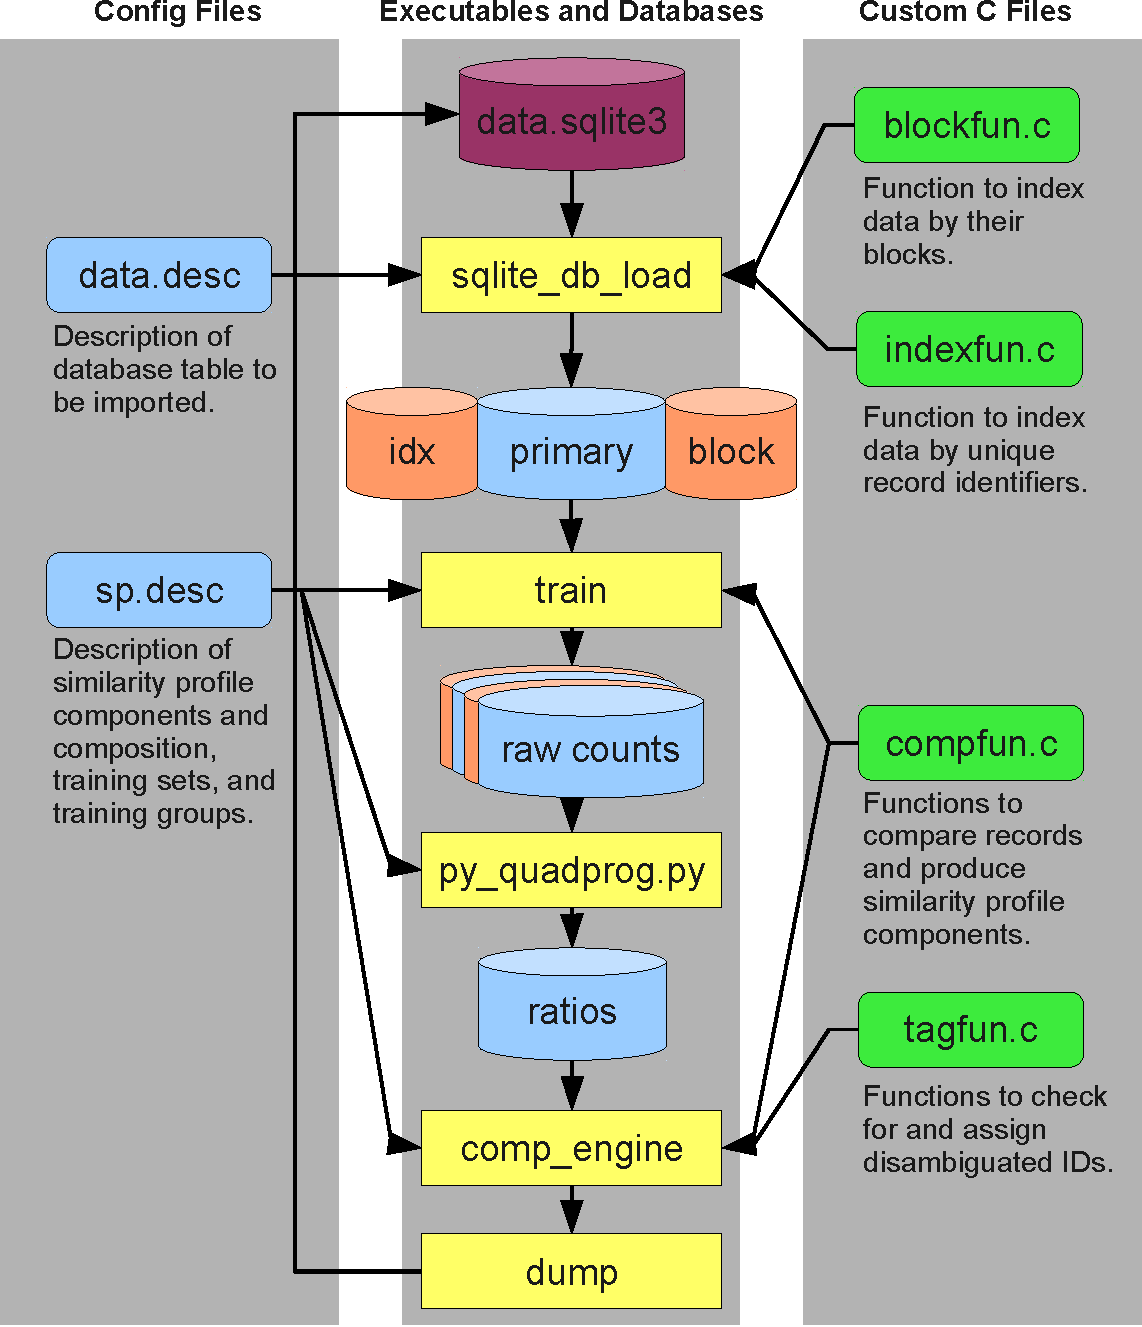
\includegraphics[scale=0.5]{Disambig_Crop.pdf}
\caption{Schematic of the disambiguation engine. Cylinders are databases, where magenta databases are sqlite databases,
blue databases are BerkeleyDB primary databases, and orange databases are BerkeleyDB secondary (index) databases. All
yellow boxes are executables, and with the exception of \texttt{py\_quadproc.py}, are compiled \texttt{C} executables.
The user should be able to customize the engine by touching only the files in the outer columns.
\label{schem}}
\end{figure}
\section{Installation}
The disambiguation engine is designed to be a standalone application to be contained and run in the same folder.
Installation is therefore really configuration, to make sure that the engine has access to the correct include
files and dynamic libraries.
\subsection{Requirements}
Below are requirements listed by type. Please make sure that your system has the following installed.
In the future, checks for these components will be automatically run by a \texttt{config} script.

\begin{verbatimtab}
Linux utilities
==============
GNU make (Included by default in most Linux distributions)

C libraries
===========
Berkeley DB >= 4.7.25
sqlite >= 3

Python Libraries and Modules
============================
Python >= 2.5
Python development files (Python.h)
CVXOPT
rpy2

R Libraries and Packages
========================
R >= 2.8
geometry
\end{verbatimtab}

\subsection{Configuration}
On an Ubuntu system, the following configuration steps are necessary to allow the engine to
locate the BerkeleyDB installation.
Some of these require the user to edit various files in the package or
system settings for installation.
Eventually, this configuration will be automatically wrapped into a \texttt{config} script.

\subsubsection{Notifying \texttt{gcc} of BerkeleyDB's location}
To compile the code, the compiler and linker in \texttt{gcc} need to know where to find BerkeleyDB
header and library files. To specify these locations, perform the following steps:
\begin{enumerate}
\item Locate the directory where BerkeleyDB was installed. This is usually under \texttt{/usr/local/bdb} or similar.
\item Edit the \texttt{Makefile} in the main directory, and set 
    \begin{itemize}
    \item \texttt{DB\_INCLUDE = /path/to/bdb/include}
    \item \texttt{DB\_LIBS = /path/to/bdb/lib}
    \end{itemize}
where they are defined at the top of the file. The default values are already included.
\item Edit \texttt{setup.py}, and set
    \begin{itemize}
    \item \texttt{DB\_INCLUDE = /path/to/bdb/include}
    \item \texttt{DB\_LIBS = /path/to/bdb/lib}
    \end{itemize}
where they are defined at the top of the file. The default values are already included.
\end{enumerate}
On many systems, the above will be enough if BerkeleyDB was installed in one of the standard library or include
paths. However, if the linker cannot find relevant include files, the following may be necessary.
\begin{itemize}
\item If you have root access:
\begin{enumerate}
\item Edit the file \texttt{/etc/ld.so.conf} or equivalent on your system, and add
    \texttt{/path/to/bdb/lib} to the bottom of the file.
\item Run \texttt{ldconfig} as root.
\end{enumerate}
\item If you do not have root access:
\begin{enumerate}
\item Set the environment variable \texttt{LD\_LIBRARY\_PATH} and append \texttt{:/path/to/bdb/lib} to the end of it.
\item To make this permanent, add the command to modify the \texttt{LD\_LIBRARY\_PATH} variable to your shell's startup files (e.g. \texttt{\textasciitilde/.bash\_profile}).
\end{enumerate}
\end{itemize}

\subsection{Using \texttt{make}}
This system is heavily reliant on the standard GNU tool \texttt{make}. The following hooks
are built into the \texttt{Makefile} to make compilation and customization easier:
\begin{itemize}
\item \texttt{all}: Compile the whole package.
\item \texttt{load}: Compile just what is necessary for \texttt{sqlite\_db\_load}.
\item \texttt{train}: Compile just what is necessary for \texttt{train}.
\item \texttt{comp}: Compile just what is necessary fo \texttt{comp\_engine}.
\item \texttt{python}: Compile and install the supporting module for \texttt{py\_quadprog.py}.
\item \texttt{clean}: Clear all non-source files from the directory.
\item \texttt{tsetclean}: Clear all training set related databases from the directory.
\item \texttt{ratioclean}: Clear the ratios database.
\end{itemize}
\section{Customization}
Customizing the database engine entails specifying the input data to the engine and
defining various parts of the training process. This is done by editing \texttt{desc} files
and by specifying \texttt{C} functions in \texttt{*fun.c} files.
\subsection{\texttt{desc} File Syntax}
As shown in Figure \ref{schem}, \texttt{desc} files in this package allow the user to
specify many database-specific aspects of the algorithm without touching \texttt{C} code.
The files are, for the most part, organized into blocks which
function like tab-delimited record listings. Each \texttt{desc} block specifies a set of
structures that will be incorporated into the \texttt{C} code, with one structure being
specified per line. Each specification takes a fixed number of fields, which are delimited
by whitespace. Each field can contain one or more entries. When a field takes multiple
entries, these entries are delimited by commas without whitespace.

A block begins with the name of the block followed (without whitespace) by an opening brace.
Specification of structures inside the block begin after a newline. A block ends with a closing
brace on its own newline following the specification of the last structure. See Figures \ref{datadesc}
and \ref{spdesc} for examples.

Lines can begin with an arbitrary amount of leading whitespace.
Lines can be commented out by starting them with a \texttt{\%} character.

The syntax here is unusually strict and will be relaxed as we make the parser her more sophisticated.
\subsection{Loading Data}
Currently, the disambiguation framework only accepts data from an sqlite3 database.
To load new data, follow these steps.
\begin{enumerate}
\item Place the sqlite3 database that contains the table that you could like to import
      into the subfolder \texttt{sqlite\_dbs}.
\item Rename the sqlite3 database \texttt{data.sqlite3}.
\item Edit the file \texttt{data.desc} in the main directory to specify your data.
\end{enumerate}
\subsubsection{\texttt{data.desc} and the \texttt{DbRecord} Structure}
The \texttt{data.desc} file specifies a sqlite query to load the raw data table and describes
that data using in a block called \texttt{data}.

The first line of \texttt{data.desc} must be the sqlite3 query, and the entire query must be contained in this first line. The first line may be followed by as many empty newlines as you like.

Records in the \texttt{data} block correspond to each column returned by the sqlite query, in the order that they are returned.
It should be noted that this block is used to define the \texttt{DbRecord} structure used in the \texttt{C} code.
Each record has two fields, in this order:
\begin{enumerate}
\item \emph{name}: This field specifies the name of the column data, and is used directly to name the field
that will store the data in the \texttt{DbRecord} structure defined in the \texttt{C} code. 
\item \emph{type}: This field specifies the type of the column data. This can take the values \texttt{unsigned\_long}, \texttt{double}, or \texttt{string(n)} which
are mapped to datatypes \texttt{u\_int32\_t}, \texttt{double}, and \texttt{char[n]}, respectively, in the \texttt{C} code.
\end{enumerate}
For an example, see Figure \ref{datadesc}. As mentioned above, the \texttt{data} block is used to define the \texttt{DbRecord} structure in the \texttt{C} code, which
you will have to use to define comparison and extraction functions in \texttt{compfun.c}. The actual \texttt{DbRecord} structure and some useful metadata
can be viewed in \texttt{sqlite\_db\_local.h} and \texttt{sqlite\_db\_local.c} after calling \texttt{make}.
\begin{figure}[!h]
\caption{An example \texttt{data.desc} file.\label{datadesc}}
\begin{verbatimtab}
select * from invpat;
%The above query returns a table with columns
%firstname, lastname, street, country, zipcode,
%lat, and lon.

data{
    %Note that there can be arbitrary leading and
    %delimiting whitespace.
    Firstname string(32)
    Lastname  string(64)
    Street    string(64)
    Country   string(3)
    Zipcode   string(6)
    Lat       double
    Lon       double
}
\end{verbatimtab}
\end{figure}

\subsection{Similarity Profile and Training Specification}
Training the disambiguation engine requires that we have a definition for the similarity profiles that will be used to calculate the likelihood that any given pair of records is actually
a match. The user needs to specify the components and levels of the similarity profile, and specify which components are trained by which training set.
To configure training, complete these steps.
\begin{enumerate}
\item Place the sqlite3 database containing the training set talbes into the subfolder \texttt{training\_sets}.
\item Rename the sqlite3 database \texttt{tset.sqlite3}.
\item Edit the file \texttt{sp.desc} in the main directory to specify the similarity profiles and traning sets.
\end{enumerate}
\subsubsection{\texttt{sp.desc}}
The \texttt{sp.desc} file provides a convenient way to specify how records will be compared and trained in one place.
Note that this file should be edited in conjunction with \texttt{compfun.c} because it will reference functions that are defined in that file.

The \texttt{sp.desc} file consists of a number of blocks each of which specifies a different aspect of the training algorithm.
Any lines that appear outside of these blocks are copied directly to \texttt{comp\_spec.h}, and can be used to specify structures and other constructs that might be useful in defining comparison functions.

\texttt{sp.desc} defines five blocks: \texttt{res\_space}, \texttt{simprof}, \texttt{match\_sets}, \texttt{nonmatch\_sets}, and \texttt{training}.
They are specified, in any order, as follows:

\paragraph{\texttt{res\_space}}
This is short for ``result space'' and refers to the levels that a comparison function can return as the result of a comparison.
Multiple comparison functions can map to the same result space, so these are defined separately.
It should be noted that this specification is used to write \texttt{typedef enum} statements to the \texttt{comp\_spec.h} file.
Each record contains the following fields in this order:
\begin{enumerate}
\item \emph{type}: The name of a result space. This will be used to define the datatype specified by the \texttt{typedef enum} statement, and will be referenced
in the \texttt{simprof} block.
\item \emph{levels}: The levels that can be returned by comparison functions that map to this result space. There should be multiple entries in this field
specified in a comma-separated list with no whitespace. The levels go from the lowest to the highest, and the names given to them should be descriptive, as this helps
greatly with debugging. This comma-separated list is copied directly into the \texttt{typedef enum} statement.
\end{enumerate}

\paragraph{\texttt{simprof}}
This is short for ``similarity profile'' and specifies various properties of the similarity profile that represents a comparison of two records.
Each record corresponds to one component of the similarity profile, and contains the following fields in this order:
\begin{enumerate}
\item \emph{type}: The type defined in \texttt{res\_space} that will populate this component of the similarity profile.
\item \emph{name}: The name that this component will take in the \texttt{simprof} structure defined in the \texttt{C} code.
\item \emph{function}: The name of the comparison function that will be used to populate this component.
Be sure that these comparison function names are consistent with the functions defined in \texttt{compfun.c}.
\item \emph{extract\_idx}: The index of the data to be extracted from the \texttt{DbRecord} structures that will be used to perform the comparisons. This will be passed as the \texttt{func\_idx} argument to the \texttt{extract} function defined in \texttt{compfun.c}.
These should be constants defined either in this file (to be copied to \texttt{comp\_spec.h}) or the \texttt{sqlite\_db\_local.h} file. See Figure \ref{spdesc} and the documentation for \texttt{compfun.c} for more details.
\item \emph{group}: The name of the training group that this component belongs to. Training groups are assumed to be independent of each other, and are trained on different sets of training sets to prevent bias. The names here will be referenced in the \texttt{training} block.
\end{enumerate}
\paragraph{\texttt{match\_sets} and \texttt{nonmatch\_sets}}
These blocks are simple listings of the match sets and non-match sets included in the \texttt{tset.sqlite3} database.
Match sets and non-match sets are specified by their table name in the database, wich one table per line.
These names will be referenced in the \texttt{training} block. 

\paragraph{\texttt{training}}
This block defines which training sets are used to train each training group.
Every training group mentioned in the \texttt{simprof} block should have a corresponding record in this block.
For each group, the training is specified as follows, in this order:
\begin{enumerate}
\item \emph{group}: The name of the training group. This should be one of the groups names mentioned in the \texttt{simprof} block.
\item \emph{match\_sets}: The name(s) of the match sets to be used to train this block. If multiple match sets are used, list the names in a comma-separated list with no whitespace.
Every match set listed here should appear in the \texttt{match\_sets} block.
\item \emph{nonmatch\_sets}: The name(s) of the non-match sets to be used. For multiples, use a comma-separated list without whitespace.
Every non-match set listed here should appear in the \texttt{nonmatch\_sets} block.
\end{enumerate}
See Figure \ref{spdesc} for an example \texttt{sp.desc} file.
\begin{figure}
\caption{An example sp.desc file.\label{spdesc}}
\begin{verbatimtab}
%%%%% This section copied directly to comp_spec.h. %%%%%
#include <math.h>
#include "strcmp95.h"

//Latitude and longitude are both used in the distance calculation, so we define
//a special extractor index and a structure that can hold them together.
#define LATLON SQLITE_DB_NUMFIELDS

typedef struct {
    double lat;
    double lon;
} latlon;

%%%%% End comp_spec.h section. %%%%%

res_space{
%   type        levels
    jwres       JWSUB75,JWMISSING,JW75,JW85,JW95,JW100
    distres     DIST100PLUS,DISTMISSING,DIST100,DIST75,DIST50,DIST10,DIST0
    coauthres   C0,C1,C2,C3,C4,C5,C6,C7,C8,C9,C10
}

simprof{
%   type        name    func        extract_idx                 group
    jwres       fname   jwcmp       SQLITE_DB_INDX_FIRSTNAME    fname       
    distres     dist    distcmp     LATLON                      loc
    coauthres   coauths coauthcmp   SQLITE_DB_INDX_COAUTHS      coauths
    %Note that multiple functions can map to the same result space.
    %Note that multiple components can use the same comparison function.
}

match_sets{
    tset01_F
    tset02_F
    tset05_F
}

nonmatch_sets{
    xset01_F
    xset03_F
}

training{
%   group       match_sets                     nonmatch_sets
    fname       tset01_F,tset05_F              xset01_F
    loc         tset02_F,tset05_F              xset03_F
    coauths     tset01_F,tset02_F              xset01_F,xset03_F
}
\end{verbatimtab}
\end{figure}
\subsection{Function Specifications}
Some parts of the disambiguation process require that we specify functions that are specific to the data
we are considering. These require that the user write their own \texttt{C} code. We have tried to pare the necessary
\texttt{C} coding down to a minimum.

Note that these \texttt{C} functions require some understanding of the BerkeleyDB C API, and of the \texttt{DbRecord} structure defined in \texttt{sqlite\_db\_local.h} following the \texttt{data.desc} configuration file.
\subsubsection{Blocking and Indexing Functions}
Blocking and indexing are performed in the disambiguation engine by the use of \emph{secondary databases}, a feature in BerkeleyDB that allows alternative methods to access records or groups of records in a database. A secondary database requires a function which it applies to every record in the database so that it can group them into appropriate buckets. For additional details on these callback functions, see the Berkeley DB C API.
\paragraph{\texttt{blockfun.c}}
This file defines the callback function used to group records together into blocks.
Those records that produce the same result from the callback function are put into the
same block, and are eligible to be compared with each other when \texttt{comp\_engine} is run.

This file must include \texttt{sqlite\_db.h}, \texttt{sqlite\_db\_local.h}, and \texttt{sqlite\_db\_extern.h}.
The function to be defined has the following prototype:
\begin{verbatimtab}
int                                 //Exit status; return 0 if successful
blocking_callback( DB* db,          //The secondary database (usually not used)
                   const DBT* key,  //The key of the database record to be blocked
                   const DBT* data, //The data of the database record to be blocked
                   DBT* result);    //The result that defines the block 
\end{verbatimtab}
\paragraph{\texttt{indexfun.c}}
The databases that are imported do not always have unique keys to identify each record.
This file allows the user to define a function that creeats a unique identifier from
each record.
This unique identifier should be used to refer to records contained in training sets, 
and should be unique for each record.

This file must include \texttt{sqlite\_db.h}, \texttt{sqlite\_db\_local.h}, and \texttt{sqlite\_db\_extern.h}.
The function to be defined has the following prototype:
\begin{verbatimtab}
int                              //Exit status; return 0 if successful
index_callback( DB* db,          //The secondary database (usually not used)
                const DBT* key,  //The key of the database record to be indexed
                const DBT* data, //The data of the database record to be indexed
                DBT* result);    //The resulting unique identifier
\end{verbatimtab}
\subsubsection{User-Defined Functions}
A core part of the disambiguation engine is comparing records on a number of different
levels to create a similarity profile. To do this, the user needs to specify custom
functions of accessing and comparing fields contained in database records. These functions include
comparison, extraction, and stop functions, and are defined in the following files.
\paragraph{\texttt{compfun.c}}
This file specifies both the \texttt{extract} function and the comparison functions mentioned in the \texttt{sp.desc} file. It must include \texttt{comp\_spec.h}.

\subparagraph{\texttt{extract}} The \texttt{extract} function is necessary because occasionally a comparison is performed using more than one field from the database records -- for example, the latitude and longitude are both used to calculate distance. The \texttt{extract} function handles both instances where you simply neeed to access one field of a \texttt{DbRecord}, and when
you need to populate and return a custom \texttt{struct} built from fileds of the \texttt{DbRecord}.

The \texttt{extract} prototye is defined as follows:
\begin{verbatimtab}
int                          //Return 1 if the return value was malloc'd
                             //and should be freed
extract( DbRecord *rp,       //Pointer to DbRecord whose field will be extracted
         const int func_idx, //Extraction index to specify which field(s) to grab
         void **result,      //Address of pointer which will reference the result
         size_t* size);      //Size of the result
\end{verbatimtab}

The extraction index \texttt{func\_idx} (soon to be renamed) is the value which determines which fields the \texttt{result} pointer will be referencing. 
If the argument to \texttt{func\_idx} is less than the number of fields in the \texttt{DbRecord} structure, then the nth field in the structure is returned.
Constants are defined in the \texttt{sqlite\_db\_local.h} file to make this referencing easy.

For special cases where the result should point to a custom data structure containing aggregate information from many fields, \texttt{func\_idx} will be an integer larger than the number of fields in a \texttt{DbRecord}.
This function should detect these cases and dynamically allocate memory for the resulting data structure.
In the cases where new memory is allocated, make sure the return value is non-zero so that the calling function knows to free the memory.
\subparagraph{\texttt{Comparison Functions}}
The comparison functions themselves are defined individually for each comparison, but have a generic prototype so that they can be stored in an array. A comparison function takes two \texttt{void} pointers and a size argument, which is the size of the bigger argument.
The comparison function is responsible for knowing what type to case the \texttt{void} pointers to before manipulating them.
The function should return an integer value which corresponds to a level that was specified in its corresponding \texttt{res\_space} in the \texttt{sp.desc} file.

The comparison function prototype is defined as follows:
\begin{verbatimtab}
int                        //Return an integer that is a valid level in the res_space
                           //specified in sp.desc for this funcion
xxxxcmp( const void* arg1, //First argument to compare (cast before manipulating)
         const void* arg2, //Second argument to compare (cast before manipulating)
         size_t size);     //Size of the larger argument
\end{verbatimtab}
\paragraph{\texttt{stopfun.c}}
Occasionally, there are conditions that are not as general as blocking which guarantee that two records could not
belong to the same entity (for example, two names that appear attached to the same document could not possibly be
the same person). In these cases, it is useful to specify a stop conditions that short-circuit the comparison, and mark
the pair with zero probability of match. This not only speeds up the computation -- it also makes the triplet correction
portion of the algorithm much more informative. Note that these conditions should only specify cases where the two records
are \emph{deterministically} incompatible, not \emph{probabilistically} incompatible, even if the condition indicates
that they are incompatible with high probability.

Stop conditions are defined in the function {\texttt{stop\_cond}}, which returns true if any of the stop
conditions indicate that the records are incompatible, and the comparison should be short-circuited. It
has the following prototype:
\begin{verbatimtab}
int                         // 1 if stop conditions are met (comparison should be stopped)
                            // 0 otherwise
stop_comp(DbRecord* db_i,   //Record to check 
          DbRecord* db_j);  //Record to check
\end{verbatimtab}

\subsubsection{Tagging (Disambiguation ID) Functions}
The ultimate point of disambiguation is to assign identifiers to records that belong to a given entity.
In this engine, the user specifies how a tag for a group is constructed, and which field in the data structure is used to store it.
\paragraph{\texttt{tagfun.c}}
This file specifies two functions which the engine uses to create and store unique entity IDs in each of the records.
\subparagraph{\texttt{has\_tag}}
The \texttt{has\_tag} function checks whether a record has already been assigned a tag. If it has one, then it returns a pointer to it;
Otherwise, it returns \texttt{NULL}. The prototype is defined as follows:
\begin{verbatimtab}
char*                           //Return a pointer to the record's tag if it has one,
                                //else, NULL.
has_tag( const DbRecord* rp );
\end{verbatimtab}
\subparagraph{\texttt{apply\_tag}}
The \texttt{apply\_tag} function assigns a tag to a particular database record. If a tag is passed in with
the record, that tag is assigned to the record. If a null pointer is passed with the record, a new tag is
created using data inside the record. The protytpe of the function is defined as follows:
\begin{verbatimtab}
int                         //Exit status
apply_tag( DbRecord *rp,    //Record to be tagged
           char *tagp);     //A string to be used as the tag, or NULL to have the
                            //create a new one.
\end{verbatimtab}
\end{document}
